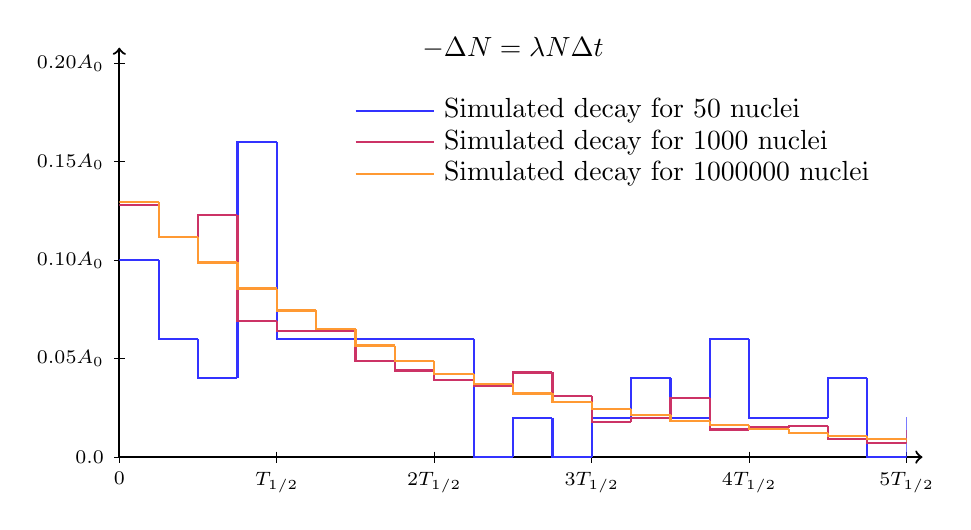
\begin{tikzpicture}
\node[] at (5.0,5.2) {$-\Delta N = \lambda N \Delta t$};
\draw[thick,->] (0.0,0.0) -- (0.0,5.2);
\draw[thick,->] (0.0,0.0) -- (10.2,0.0);
\draw (0,0cm + 2pt) -- (0, 0cm-2pt) node[below] {\scriptsize $0$};
\draw (2,0cm + 2pt) -- (2, 0cm-2pt) node[below] {\scriptsize $T_{1/2}$};
\draw (4,0cm + 2pt) -- (4, 0cm-2pt) node[below] {\scriptsize $2T_{1/2}$};
\draw (6,0cm + 2pt) -- (6, 0cm-2pt) node[below] {\scriptsize $3T_{1/2}$};
\draw (8,0cm + 2pt) -- (8, 0cm-2pt) node[below] {\scriptsize $4T_{1/2}$};
\draw (10,0cm + 2pt) -- (10, 0cm-2pt) node[below] {\scriptsize $5T_{1/2}$};
\draw (0cm+2pt,0.    ) -- (0cm-2pt,0.    ) node[left] {\scriptsize $0.0$};
\draw (0cm+2pt,1.25    ) -- (0cm-2pt,1.25    ) node[left] {\scriptsize $0.05 A_0$};
\draw (0cm+2pt,2.5    ) -- (0cm-2pt,2.5    ) node[left] {\scriptsize $0.10 A_0$};
\draw (0cm+2pt,3.750000093132256    ) -- (0cm-2pt,3.750000093132256    ) node[left] {\scriptsize $0.15 A_0$};
\draw (0cm+2pt,5.    ) -- (0cm-2pt,5.    ) node[left] {\scriptsize $0.20 A_0$};
\begin{scope}[]
\clip (0,0) rectangle (10,5);
\draw[blue!80,thick] (3.0,4.4) -- (4.0,4.4);
\node[right,] at (4.0,4.4) {Simulated decay for 50 nuclei};
\begin{scope}[blue!80,thick]
\draw[] (0.0,2.4999999627470975) -- (0.5,2.4999999627470975);
\draw (0.5,2.4999999627470975) -- (0.5,1.4999999776482584) -- (1.0,1.4999999776482584);
\draw (1.0,1.4999999776482584) -- (1.0,0.999999985098839) -- (1.5,0.999999985098839);
\draw (1.5,0.999999985098839) -- (1.5,3.999999940395356) -- (2.0,3.999999940395356);
\draw (2.0,3.999999940395356) -- (2.0,1.4999999776482584) -- (2.5,1.4999999776482584);
\draw (2.5,1.4999999776482584) -- (2.5,1.4999999776482584) -- (3.0,1.4999999776482584);
\draw (3.0,1.4999999776482584) -- (3.0,1.4999999776482584) -- (3.5,1.4999999776482584);
\draw (3.5,1.4999999776482584) -- (3.5,1.4999999776482584) -- (4.0,1.4999999776482584);
\draw (4.0,1.4999999776482584) -- (4.0,1.4999999776482584) -- (4.5,1.4999999776482584);
\draw (4.5,1.4999999776482584) -- (4.5,0.0) -- (5.0,0.0);
\draw (5.0,0.0) -- (5.0,0.4999999925494195) -- (5.5,0.4999999925494195);
\draw (5.5,0.4999999925494195) -- (5.5,0.0) -- (6.0,0.0);
\draw (6.0,0.0) -- (6.0,0.4999999925494195) -- (6.5,0.4999999925494195);
\draw (6.5,0.4999999925494195) -- (6.5,0.999999985098839) -- (7.0,0.999999985098839);
\draw (7.0,0.999999985098839) -- (7.0,0.4999999925494195) -- (7.5,0.4999999925494195);
\draw (7.5,0.4999999925494195) -- (7.5,1.4999999776482584) -- (8.0,1.4999999776482584);
\draw (8.0,1.4999999776482584) -- (8.0,0.4999999925494195) -- (8.5,0.4999999925494195);
\draw (8.5,0.4999999925494195) -- (8.5,0.4999999925494195) -- (9.0,0.4999999925494195);
\draw (9.0,0.4999999925494195) -- (9.0,0.999999985098839) -- (9.5,0.999999985098839);
\draw (9.5,0.999999985098839) -- (9.5,0.0) -- (10.0,0.0);
\draw (10.0,0.0) -- (10.0,0.4999999925494195) -- (10.5,0.4999999925494195);
\draw (10.5,0.4999999925494195) -- (10.5,0.0) -- (11.0,0.0);
\draw (11.0,0.0) -- (11.0,0.0) -- (11.5,0.0);
\draw (11.5,0.0) -- (11.5,0.999999985098839) -- (12.0,0.999999985098839);
\draw (12.0,0.999999985098839) -- (12.0,0.0) -- (12.5,0.0);
\end{scope}
\draw[purple!80,thick] (3.0,4.0) -- (4.0,4.0);
\node[right,] at (4.0,4.0) {Simulated decay for 1000 nuclei};
\begin{scope}[purple!80,thick]
\draw[] (0.0,3.199999952316285) -- (0.5,3.199999952316285);
\draw (0.5,3.199999952316285) -- (0.5,2.799999958276749) -- (1.0,2.799999958276749);
\draw (1.0,2.799999958276749) -- (1.0,3.0749999541789297) -- (1.5,3.0749999541789297);
\draw (1.5,3.0749999541789297) -- (1.5,1.7249999742954973) -- (2.0,1.7249999742954973);
\draw (2.0,1.7249999742954973) -- (2.0,1.5999999761581425) -- (2.5,1.5999999761581425);
\draw (2.5,1.5999999761581425) -- (2.5,1.5999999761581425) -- (3.0,1.5999999761581425);
\draw (3.0,1.5999999761581425) -- (3.0,1.2249999817460777) -- (3.5,1.2249999817460777);
\draw (3.5,1.2249999817460777) -- (3.5,1.0999999836087229) -- (4.0,1.0999999836087229);
\draw (4.0,1.0999999836087229) -- (4.0,0.974999985471368) -- (4.5,0.974999985471368);
\draw (4.5,0.974999985471368) -- (4.5,0.8999999865889551) -- (5.0,0.8999999865889551);
\draw (5.0,0.8999999865889551) -- (5.0,1.0749999839812518) -- (5.5,1.0749999839812518);
\draw (5.5,1.0749999839812518) -- (5.5,0.7749999884516002) -- (6.0,0.7749999884516002);
\draw (6.0,0.7749999884516002) -- (6.0,0.44999999329447754) -- (6.5,0.44999999329447754);
\draw (6.5,0.44999999329447754) -- (6.5,0.4999999925494195) -- (7.0,0.4999999925494195);
\draw (7.0,0.4999999925494195) -- (7.0,0.7499999888241292) -- (7.5,0.7499999888241292);
\draw (7.5,0.7499999888241292) -- (7.5,0.34999999478459365) -- (8.0,0.34999999478459365);
\draw (8.0,0.34999999478459365) -- (8.0,0.3749999944120646) -- (8.5,0.3749999944120646);
\draw (8.5,0.3749999944120646) -- (8.5,0.3999999940395356) -- (9.0,0.3999999940395356);
\draw (9.0,0.3999999940395356) -- (9.0,0.22499999664723877) -- (9.5,0.22499999664723877);
\draw (9.5,0.22499999664723877) -- (9.5,0.17499999739229682) -- (10.0,0.17499999739229682);
\draw (10.0,0.17499999739229682) -- (10.0,0.32499999515712263) -- (10.5,0.32499999515712263);
\draw (10.5,0.32499999515712263) -- (10.5,0.24999999627470976) -- (11.0,0.24999999627470976);
\draw (11.0,0.24999999627470976) -- (11.0,0.07499999888241293) -- (11.5,0.07499999888241293);
\draw (11.5,0.07499999888241293) -- (11.5,0.04999999925494195) -- (12.0,0.04999999925494195);
\draw (12.0,0.04999999925494195) -- (12.0,0.07499999888241293) -- (12.5,0.07499999888241293);
\end{scope}
\draw[orange!80,thick] (3.0,3.6) -- (4.0,3.6);
\node[right,] at (4.0,3.6) {Simulated decay for 1000000 nuclei};
\begin{scope}[orange!80,thick]
\draw[] (0.0,3.2356499517850588) -- (0.5,3.2356499517850588);
\draw (0.5,3.2356499517850588) -- (0.5,2.797074958320335) -- (1.0,2.797074958320335);
\draw (1.0,2.797074958320335) -- (1.0,2.4715999631702905) -- (1.5,2.4715999631702905);
\draw (1.5,2.4715999631702905) -- (1.5,2.140674968101457) -- (2.0,2.140674968101457);
\draw (2.0,2.140674968101457) -- (2.0,1.862524972246215) -- (2.5,1.862524972246215);
\draw (2.5,1.862524972246215) -- (2.5,1.6247499757893389) -- (3.0,1.6247499757893389);
\draw (3.0,1.6247499757893389) -- (3.0,1.4168499788872901) -- (3.5,1.4168499788872901);
\draw (3.5,1.4168499788872901) -- (3.5,1.2253999817401173) -- (4.0,1.2253999817401173);
\draw (4.0,1.2253999817401173) -- (4.0,1.0530499843083323) -- (4.5,1.0530499843083323);
\draw (4.5,1.0530499843083323) -- (4.5,0.9316749861169609) -- (5.0,0.9316749861169609);
\draw (5.0,0.9316749861169609) -- (5.0,0.8082999879553916) -- (5.5,0.8082999879553916);
\draw (5.5,0.8082999879553916) -- (5.5,0.7001749895665796) -- (6.0,0.7001749895665796);
\draw (6.0,0.7001749895665796) -- (6.0,0.6116499908857049) -- (6.5,0.6116499908857049);
\draw (6.5,0.6116499908857049) -- (6.5,0.5331749920550735) -- (7.0,0.5331749920550735);
\draw (7.0,0.5331749920550735) -- (7.0,0.4615999931216241) -- (7.5,0.4615999931216241);
\draw (7.5,0.4615999931216241) -- (7.5,0.40359999398589136) -- (8.0,0.40359999398589136);
\draw (8.0,0.40359999398589136) -- (8.0,0.3537249947290868) -- (8.5,0.3537249947290868);
\draw (8.5,0.3537249947290868) -- (8.5,0.3068999954268337) -- (9.0,0.3068999954268337);
\draw (9.0,0.3068999954268337) -- (9.0,0.27094999596253044) -- (9.5,0.27094999596253044);
\draw (9.5,0.27094999596253044) -- (9.5,0.232974996528402) -- (10.0,0.232974996528402);
\draw (10.0,0.232974996528402) -- (10.0,0.20547499693818397) -- (10.5,0.20547499693818397);
\draw (10.5,0.20547499693818397) -- (10.5,0.17442499740086498) -- (11.0,0.17442499740086498);
\draw (11.0,0.17442499740086498) -- (11.0,0.1518499977372587) -- (11.5,0.1518499977372587);
\draw (11.5,0.1518499977372587) -- (11.5,0.13397499800361695) -- (12.0,0.13397499800361695);
\draw (12.0,0.13397499800361695) -- (12.0,0.11737499825097623) -- (12.5,0.11737499825097623);
\end{scope}
\end{scope}
\end{tikzpicture}
%%% Local Variables: 
%%% mode: latex 
%%% TeX-master: "master" 
%%% End:

